% ============================================================
%  MUTUAL FUNDS: A VISUAL BEGINNER'S GUIDE  v2.0
%  Improved readability, updated tax rates (Budget 2024)
% ============================================================
\documentclass[11pt,a4paper]{article}

% --- Core layout ---
\usepackage[top=1.8cm,bottom=1.8cm,left=1.8cm,right=1.8cm]{geometry}
\usepackage{multicol}
\usepackage{parskip}
\setlength{\parskip}{5pt}
\setlength{\columnsep}{14pt}

% --- Fonts & encoding ---
\usepackage[T1]{fontenc}
\usepackage[utf8]{inputenc}
\usepackage{lmodern}
\usepackage{microtype}
% Rupee symbol workaround (no tfrupee installed)
\DeclareUnicodeCharacter{20B9}{\textbf{\textsf{Rs.}}}
\newcommand{\rupee}{\textbf{\textsf{Rs.}}}

% --- Color ---
\usepackage[dvipsnames,svgnames,x11names]{xcolor}
\definecolor{primary}{HTML}{1A3A5C}
\definecolor{accent}{HTML}{E8A020}
\definecolor{accent2}{HTML}{2196A6}
\definecolor{positive}{HTML}{2E7D32}
\definecolor{negative}{HTML}{C62828}
\definecolor{warning}{HTML}{E65100}
\definecolor{lightbg}{HTML}{F4F7FA}
\definecolor{lightaccent}{HTML}{FFF8E1}
\definecolor{lightgreen}{HTML}{E8F5E9}
\definecolor{lightred}{HTML}{FFEBEE}
\definecolor{lightteal}{HTML}{E0F4F6}
\definecolor{cardbg}{HTML}{FAFBFC}

% --- Graphics & diagrams ---
\usepackage{tikz}
\usepackage{pgfplots}
\pgfplotsset{compat=1.18}
\usetikzlibrary{shapes.geometric, arrows.meta, positioning, calc, fit,
                shadows, backgrounds, patterns, mindmap, trees}

% --- Tables ---
\usepackage{booktabs}
\usepackage{array}
\usepackage{colortbl}
\usepackage{tabularx}
\usepackage{multirow}

% --- Boxes & frames ---
\usepackage[most]{tcolorbox}
\tcbuselibrary{skins,breakable,listings}

% --- Lists ---
\usepackage{enumitem}
\setlist{nosep, leftmargin=1.4em}
\setlist[itemize]{label={\color{accent}$\bullet$}}

% --- Headers & section styling ---
\usepackage[explicit]{titlesec}
\usepackage{fancyhdr}
\usepackage{pifont}
\usepackage{wasysym}

% --- PDF features ---
\usepackage[colorlinks=true, linkcolor=primary, urlcolor=accent2]{hyperref}

% ============================================================
% SECTION STYLING
% ============================================================
\titleformat{\section}
  {\color{primary}\Large\bfseries\sffamily}
  {\colorbox{primary}{\textcolor{white}{\thesection}}}{0.6em}{#1}
  [{\color{accent}\hrule height 1.5pt}]

\titleformat{\subsection}
  {\color{primary}\normalsize\bfseries\sffamily}
  {}{0em}{\colorbox{accent!20}{\strut\quad#1\quad}}[]

\titlespacing{\section}{0pt}{12pt}{7pt}
\titlespacing{\subsection}{0pt}{9pt}{5pt}

% ============================================================
% TCOLORBOX STYLES
% ============================================================
\newtcolorbox{keybox}[1][]{%
  enhanced, breakable, colback=lightbg, colframe=primary, arc=3pt,
  boxrule=1.2pt, left=7pt, right=7pt, top=5pt, bottom=5pt,
  fonttitle=\small\bfseries\sffamily\color{white},
  attach boxed title to top left={yshift=-2mm, xshift=6mm},
  boxed title style={colback=primary, arc=2pt, boxrule=0pt}, #1}

\newtcolorbox{tipbox}[1][]{%
  enhanced, colback=lightaccent, colframe=accent, arc=3pt,
  boxrule=1pt, left=7pt, right=7pt, top=5pt, bottom=5pt,
  fonttitle=\small\bfseries\sffamily\color{white},
  attach boxed title to top left={yshift=-2mm, xshift=6mm},
  boxed title style={colback=accent, arc=2pt, boxrule=0pt}, #1}

\newtcolorbox{warnbox}[1][]{%
  enhanced, colback=lightred, colframe=negative, arc=3pt,
  boxrule=1pt, left=7pt, right=7pt, top=5pt, bottom=5pt,
  fonttitle=\small\bfseries\sffamily\color{white},
  attach boxed title to top left={yshift=-2mm, xshift=6mm},
  boxed title style={colback=negative, arc=2pt, boxrule=0pt}, #1}

\newtcolorbox{infobox}[1][]{%
  enhanced, colback=lightteal, colframe=accent2, arc=3pt,
  boxrule=1pt, left=7pt, right=7pt, top=5pt, bottom=5pt,
  fonttitle=\small\bfseries\sffamily\color{white},
  attach boxed title to top left={yshift=-2mm, xshift=6mm},
  boxed title style={colback=accent2, arc=2pt, boxrule=0pt}, #1}

% ============================================================
% HELPER COMMANDS
% ============================================================
\newcommand{\pro}[1]{\textcolor{positive}{\ding{52}\,}#1}
\newcommand{\con}[1]{\textcolor{negative}{\ding{56}\,}#1}

% ============================================================
% PAGE STYLE
% ============================================================
\pagestyle{fancy}
\fancyhf{}
\fancyhead[L]{\small\color{primary}\sffamily\textbf{Mutual Funds: A Visual Beginner's Guide}}
\fancyhead[R]{\small\color{accent2}\sffamily Indian Market Edition \textemdash\ v2.0}
\fancyfoot[C]{\small\color{primary!60}\thepage}
\setlength{\headheight}{20pt}
\renewcommand{\headrulewidth}{0.4pt}
\renewcommand{\headrule}{{\color{primary!40}\hrule height 0.4pt width\headwidth}}

% ============================================================
\begin{document}
% ============================================================

% ============================================================
% COVER PAGE
% ============================================================
\thispagestyle{empty}
\begin{tikzpicture}[remember picture, overlay]
  \fill[primary] (current page.south west) rectangle (current page.north east);
  \fill[accent] (current page.north west) rectangle +(\paperwidth,-0.85cm);
  \fill[accent2] (current page.south west) rectangle +(\paperwidth,0.55cm);
  \fill[white,opacity=0.04] ([xshift=10cm,yshift=5cm]current page.south west) circle (9cm);
  \fill[white,opacity=0.04] ([xshift=2cm,yshift=15cm]current page.south west) circle (6cm);

  \node[anchor=north, text=white, font=\fontsize{38}{44}\selectfont\bfseries\sffamily,
        text width=17cm, align=center]
    at ([yshift=-2.8cm]current page.north) {MUTUAL FUNDS};

  \node[anchor=north, text=accent, font=\fontsize{20}{24}\selectfont\sffamily,
        text width=17cm, align=center]
    at ([yshift=-5.4cm]current page.north) {A Visual Beginner's Guide};

  \node[anchor=north, text=white!75, font=\fontsize{12}{15}\selectfont\sffamily,
        text width=15cm, align=center]
    at ([yshift=-7.2cm]current page.north)
    {From Zero to Informed Investor \textemdash\ Indian Market Edition};

  % Growth curve diagram
  \begin{scope}[shift={([yshift=2.2cm]current page.center)}, xscale=1.2]
    \draw[white,opacity=0.12,line width=0.8pt] (-6,-2) grid[step=1] (6,4);
    \draw[accent, line width=3pt, rounded corners=2pt]
      (-5,-1.5) to[out=35,in=205] (0,0.5)
      to[out=25,in=210] (3,2)
      to[out=35,in=225] (5,4.5);
    \fill[accent] (5,4.5) circle (6pt);
    \node[text=accent, font=\small\sffamily\bfseries, anchor=west] at (5.15,4.5) {Wealth};
    \draw[accent2!80, line width=1.5pt, dashed] (-5,-1) -- (5, 0.5);
    \node[text=accent2!80, font=\footnotesize\sffamily, anchor=west] at (5.15,0.5) {Inflation};
    \node[text=white!50, font=\tiny\sffamily] at (-4.5,-1.8) {Time \textrightarrow};
  \end{scope}

  % Bottom tagline
  \node[text=white!70, font=\small\sffamily, align=center]
    at ([yshift=1.3cm]current page.south)
    {\textbf{Covers:} Fund Types $\cdot$ Risk Metrics $\cdot$ Portfolio Building $\cdot$ SIP Strategy $\cdot$ Tax (Updated: Budget 2024)};
\end{tikzpicture}

\newpage

% ============================================================
% LEARNING JOURNEY
% ============================================================

\begin{tikzpicture}
  \fill[primary] (0,0) rectangle (\linewidth, 0.75cm);
  \node[text=white, font=\large\bfseries\sffamily, anchor=west] at (0.3,0.375)
    {\ding{73}~Your Learning Journey};
\end{tikzpicture}

\vspace{5pt}
\begin{tikzpicture}[node distance=0cm, scale=0.88, transform shape]
  \tikzstyle{journeystep}=[rectangle, rounded corners=5pt, minimum width=2.4cm,
    minimum height=1.1cm, text centered, font=\footnotesize\sffamily\bfseries,
    draw, line width=1pt]
  \tikzstyle{arr}=[-{Stealth[length=5pt]}, line width=1.3pt, color=primary!50]
  \node[journeystep, fill=primary!15, draw=primary] (s1) at (0,0)
    {\textcolor{primary}{1. What \&}\\\textcolor{primary}{Why MFs}};
  \node[journeystep, fill=accent!15, draw=accent] (s2) [right=0.5cm of s1]
    {\textcolor{warning}{2. Fund}\\\textcolor{warning}{Types}};
  \node[journeystep, fill=accent2!15, draw=accent2] (s3) [right=0.5cm of s2]
    {\textcolor{accent2}{3. Key}\\\textcolor{accent2}{Metrics}};
  \node[journeystep, fill=positive!10, draw=positive] (s4) [right=0.5cm of s3]
    {\textcolor{positive}{4. Select}\\\textcolor{positive}{the Fund}};
  \node[journeystep, fill=primary!15, draw=primary] (s5) [right=0.5cm of s4]
    {\textcolor{primary}{5. Build}\\\textcolor{primary}{Portfolio}};
  \node[journeystep, fill=accent!15, draw=accent] (s6) [right=0.5cm of s5]
    {\textcolor{warning}{6. Manage}\\\textcolor{warning}{\& Grow}};
  \draw[arr] (s1.east) -- (s2.west);
  \draw[arr] (s2.east) -- (s3.west);
  \draw[arr] (s3.east) -- (s4.west);
  \draw[arr] (s4.east) -- (s5.west);
  \draw[arr] (s5.east) -- (s6.west);
\end{tikzpicture}

\vspace{7pt}

% ============================================================
% SECTION 1: WHAT IS A MUTUAL FUND
% ============================================================
\section{What is a Mutual Fund \& Why Invest?}

\begin{multicols}{2}

\begin{keybox}[title=The Core Idea]
A \textbf{mutual fund} pools money from many investors and a professional \textbf{fund manager} invests it in a diversified basket of stocks, bonds, or other assets on your behalf. You own \textbf{units} of the fund; the fund's value per unit is called the \textbf{NAV} (Net Asset Value).
\end{keybox}

\textbf{The problem with alternatives:}
\begin{itemize}
  \item \textbf{FDs / Government schemes} --- often beaten by inflation after tax
  \item \textbf{Direct stock picking} --- emotional, time-consuming, high skill needed
  \item \textbf{Insurance products} --- your money still goes to markets; they keep the alpha
\end{itemize}

\columnbreak

\begin{center}
\begin{tikzpicture}[
  every node/.style={font=\sffamily},
  investor/.style={circle, fill=primary!12, draw=primary!35, minimum size=0.56cm,
                   inner sep=0pt, font=\scriptsize\bfseries\sffamily, text=primary},
  invlabel/.style={text=primary!85, font=\tiny\sffamily, align=center},
  pool/.style={rectangle, rounded corners=3pt, draw=accent!70, fill=accent!18,
               minimum width=3.20cm, minimum height=0.62cm, align=center,
               font=\scriptsize\bfseries\sffamily, text=primary},
  manager/.style={rectangle, rounded corners=3pt, draw=primary!85, fill=primary!85,
                  text=white, minimum width=3.25cm, minimum height=0.72cm,
                  align=center, font=\scriptsize\bfseries\sffamily},
  asset/.style={rectangle, rounded corners=2pt, draw=#1!70, fill=#1!18,
                minimum width=1.05cm, minimum height=0.46cm, align=center,
                inner sep=1.5pt, font=\tiny\sffamily, text=primary},
  flow/.style={-{Stealth[length=4pt]}, primary!60, line width=0.8pt},
  ret/.style={rectangle, rounded corners=3pt, draw=positive!60, fill=positive!12,
              text=positive!70!black, minimum width=3.80cm, align=center,
              font=\scriptsize\bfseries\sffamily, inner sep=3pt}
]
  \node[investor] (i1) at (0.0, 4.05) {I1};
  \node[investor] (i2) at (1.65, 4.05) {I2};
  \node[investor] (i3) at (3.30, 4.05) {I3};
  \node[invlabel, above=2pt of i1] {Investor 1};
  \node[invlabel, above=2pt of i2] {Investor 2};
  \node[invlabel, above=2pt of i3] {Investor 3};

  \node[pool] (pool) at (1.65, 2.90) {POOLED MONEY};
  \node[manager] (mgr) at (1.65, 1.88) {Fund Manager\\(AMC)};
  \node[asset=positive] (stk) at (0.20, 0.78) {Stocks};
  \node[asset=accent2] (bnd) at (1.65, 0.78) {Bonds};
  \node[asset=warning] (oth) at (3.10, 0.78) {Others};
  \node[ret] (nav) at (1.65, -0.10) {NAV grows $\rightarrow$ returns};

  \draw[flow] (i1.south) -- (pool.north west);
  \draw[flow] (i2.south) -- (pool.north);
  \draw[flow] (i3.south) -- (pool.north east);
  \node[text=primary!60, font=\tiny\sffamily, fill=white, inner sep=1pt]
    at (1.65, 3.52) {investments};

  \draw[flow] (pool.south) -- node[right, text=primary!60, font=\tiny\sffamily] {units} (mgr.north);
  \draw[flow] (mgr.south west) -- (stk.north);
  \draw[flow] (mgr.south) -- node[right, text=primary!60, font=\tiny\sffamily] {allocates} (bnd.north);
  \draw[flow] (mgr.south east) -- (oth.north);
  \draw[-{Stealth[length=4pt]}, positive!70, line width=0.8pt, dashed] (stk.south) -- (nav.north west);
  \draw[-{Stealth[length=4pt]}, positive!70, line width=0.8pt, dashed] (bnd.south) -- (nav.north);
  \draw[-{Stealth[length=4pt]}, positive!70, line width=0.8pt, dashed] (oth.south) -- (nav.north east);
\end{tikzpicture}
\end{center}

\end{multicols}

\textbf{Why mutual funds work for most investors:}
\vspace{4pt}


\begin{tikzpicture}[every node/.style={font=\sffamily}]
\tikzstyle{benefit}=[rectangle, rounded corners=5pt, fill=lightbg, draw=primary!30,
  minimum height=1.5cm, text width=2.65cm, align=center, font=\scriptsize\sffamily]
\node[benefit] (b1) at (0,0)
  {\textcolor{primary}{\bfseries\small Professional}\\\textcolor{primary}{\bfseries\small Management}\\Expert decisions for you};
\node[benefit] (b2) at (2.9,0)
  {\textcolor{accent2}{\bfseries\small Diversification}\\Risk spread across\\many assets};
\node[benefit] (b3) at (5.8,0)
  {\textcolor{positive}{\bfseries\small Liquidity}\\Redeem any\\business day};
\node[benefit] (b4) at (8.7,0)
  {\textcolor{warning}{\bfseries\small Accessibility}\\Start with just\\\rupee{}500 per month};
\node[benefit] (b5) at (11.6,0)
  {\textcolor{primary}{\bfseries\small Transparency}\\SEBI-regulated,\\monthly disclosures};
\end{tikzpicture}

\vspace{5pt}
\begin{tipbox}[title=The Compounding Magic]
\textbf{\rupee{}5,000/month at 12\% CAGR over 30 years = \rupee{}1.75 crore.}  The same amount in an FD at 6\% gives roughly \rupee{}50 lakh.  Time is your most powerful asset --- start early and stay invested.
\end{tipbox}

% ============================================================
% SECTION 2: TYPES OF FUNDS
% ============================================================
\section{Types of Mutual Funds}

\subsection{The Big Three by Asset Class}

\begin{tikzpicture}[every node/.style={font=\sffamily}]
  % EQUITY
  \fill[primary!90, rounded corners=6pt] (0,0) rectangle (4.6, 5.1);
  \node[text=white, font=\bfseries\large\sffamily, align=center] at (2.3, 4.72)
    {EQUITY FUNDS};
  \node[text=white!88, font=\footnotesize\sffamily, align=center, text width=4.3cm]
    at (2.3, 3.95) {Invest in company stocks\\Min 65\% in equities (SEBI)};
  \node[anchor=north west, text=white, align=left, text width=4.1cm,
        font=\footnotesize\sffamily] at (0.25, 3.18)
    {\textcolor{lightgreen}{\ding{52}}\,High long-term returns\\[2pt]
     \textcolor{lightgreen}{\ding{52}}\,Beats inflation comfortably\\[2pt]
     \textcolor{lightred}{\ding{56}}\,High short-term volatility\\[2pt]
     \textcolor{lightred}{\ding{56}}\,Needs 5+ year horizon};
  \node[text=accent, font=\bfseries\footnotesize\sffamily] at (2.3, 0.45)
    {RISK: {\color{lightred}\large HIGH}};

  % DEBT
  \fill[accent2!80, rounded corners=6pt] (5.0,0) rectangle (9.6, 5.1);
  \node[text=white, font=\bfseries\large\sffamily, align=center] at (7.3, 4.72)
    {DEBT FUNDS};
  \node[text=white!90, font=\footnotesize\sffamily, align=center, text width=4.3cm]
    at (7.3, 3.95) {Invest in bonds \& fixed-income\\instruments};
  \node[anchor=north west, text=white, align=left, text width=4.1cm,
        font=\footnotesize\sffamily] at (5.25, 3.18)
    {\textcolor{lightgreen}{\ding{52}}\,Stable returns (6--9\%)\\[2pt]
     \textcolor{lightgreen}{\ding{52}}\,Good for short/medium goals\\[2pt]
     \textcolor{lightred}{\ding{56}}\,Lower returns than equity\\[2pt]
     \textcolor{lightred}{\ding{56}}\,Credit \& interest-rate risk};
  \node[text=white, font=\bfseries\footnotesize\sffamily] at (7.3, 0.45)
    {RISK: {\color{accent}\large MEDIUM}};

  % HYBRID
  \fill[positive!70, rounded corners=6pt] (10.0,0) rectangle (14.6, 5.1);
  \node[text=white, font=\bfseries\large\sffamily, align=center] at (12.3, 4.72)
    {HYBRID FUNDS};
  \node[text=white!92, font=\footnotesize\sffamily, align=center, text width=4.3cm]
    at (12.3, 3.95) {Mix of equity + debt\\Balanced risk-return};
  \node[anchor=north west, text=white, align=left, text width=4.1cm,
        font=\footnotesize\sffamily] at (10.25, 3.18)
    {\textcolor{lightgreen}{\ding{52}}\,Built-in diversification\\[2pt]
     \textcolor{lightgreen}{\ding{52}}\,Suits moderate risk tolerance\\[2pt]
     \textcolor{lightred}{\ding{56}}\,Manager-dependent balance\\[2pt]
     \textcolor{lightred}{\ding{56}}\,Higher expense than pure funds};
  \node[text=white, font=\bfseries\footnotesize\sffamily] at (12.3, 0.45)
    {RISK: {\color{lightgreen}\large LOW--MED}};
\end{tikzpicture}

\vspace{8pt}
\subsection{Equity Fund Sub-Categories (SEBI 2017 Classification)}

\begin{tabularx}{\linewidth}{|>{\bfseries\small\sffamily}p{3.2cm}|>{\small}X|>{\small\centering\arraybackslash}p{2.4cm}|>{\small\centering\arraybackslash}p{2.1cm}|}
\hline
\rowcolor{primary!90}[0pt][0pt]
\textcolor{white}{\small Fund Category} & \textcolor{white}{\small Who It Invests In} &
\textcolor{white}{\small Ideal Horizon} & \textcolor{white}{\small Risk} \\
\hline
\rowcolor{lightbg}[0pt][0pt]
Large Cap & Top 100 companies by market cap (min 80\%) & 5--7 years & \textcolor{warning}{Moderate} \\
\hline
Mid Cap & Rank 101--250 companies (min 65\%) & 7--10 years & \textcolor{negative}{High} \\
\hline
\rowcolor{lightbg}[0pt][0pt]
Small Cap & Rank 251+ companies (min 65\%) & 10+ years & \textcolor{negative}{\bfseries Very High} \\
\hline
Flexi Cap & Any market cap, dynamically (min 65\% equity) & 7+ years & \textcolor{negative}{High} \\
\hline
\rowcolor{lightbg}[0pt][0pt]
Large \& Mid Cap & Min 35\% large + min 35\% mid & 7+ years & \textcolor{negative}{High} \\
\hline
Multi Cap & Min 25\% each: large, mid, small & 7+ years & \textcolor{negative}{High} \\
\hline
\rowcolor{lightbg}[0pt][0pt]
ELSS & Min 80\% equity + 3-yr lock-in + 80C tax benefit & 3+ years & \textcolor{negative}{High} \\
\hline
Index Fund & Tracks Nifty/Sensex passively & 5+ years & \textcolor{warning}{Moderate} \\
\hline
\rowcolor{lightbg}
Sectoral/Thematic & Single sector (IT, pharma, etc.) min 80\% & 7+ years & \textcolor{negative}{\bfseries Very High} \\
\hline
\end{tabularx}

\vspace{7pt}
\subsection{Debt Fund Sub-Categories (by Duration)}

\begin{center}
\begin{tikzpicture}[
  every node/.style={font=\sffamily},
  laddertext/.style={text=primary, font=\scriptsize\sffamily, align=center, text width=3.45cm},
  ladderline/.style={line width=1.1pt, -{Stealth[length=5pt]}}
]
  \def\cw{3.80}
  \def\ch{1.92}

  % Direction arrows
  \draw[ladderline, negative!75] (0, 4.16) -- (15.95, 4.16);
  \node[text=negative!80, font=\footnotesize\bfseries\sffamily, align=center]
    at (7.98, 4.43) {Interest-rate sensitivity and NAV swings increase};
  \draw[ladderline, positive!75] (15.95, 3.74) -- (0, 3.74);
  \node[text=positive!70!black, font=\footnotesize\bfseries\sffamily, align=center]
    at (7.98, 3.50) {Liquidity and capital safety increase};

  % Macro to draw one duration card
  % Args: x_start, y_start, color, title, bold_line1, body_line, risk_label
  \newcommand{\dcard}[7]{%
    \pgfmathsetmacro{\xm}{#1 + \cw/2}
    \pgfmathsetmacro{\titlex}{#1 + 0.07}
    \pgfmathsetmacro{\titley}{#2 + \ch - 0.40}
    \pgfmathsetmacro{\titlew}{\cw - 0.14}
    \pgfmathsetmacro{\titlemid}{#2 + \ch - 0.20}
    \fill[#3!9, draw=#3!75, line width=0.9pt, rounded corners=4pt]
      (#1,#2) rectangle ++(\cw,\ch);
    \fill[#3!80, rounded corners=3pt]
      (\titlex,\titley) rectangle ++(\titlew,0.34);
    \node[text=white, font=\footnotesize\bfseries\sffamily, align=center, text width=3.45cm]
      at (\xm,\titlemid) {#4};
    \node[text=#3!90!black, font=\scriptsize\bfseries\sffamily, align=center, text width=3.45cm]
      at (\xm,#2+1.12) {#5};
    \node[laddertext] at (\xm,#2+0.70) {#6};
    \node[text=#3!85!black, font=\scriptsize\bfseries\sffamily, align=center, text width=3.45cm]
      at (\xm,#2+0.28) {#7};
  }

  % Row 1 (top, lower risk)
  \dcard{0.00}{1.36}{positive}{Overnight}{Duration: 1 day}
    {Use: idle cash}{Lowest volatility}
  \dcard{4.05}{1.36}{positive}{Liquid}{Maturity: up to 91 days}
    {Use: emergency fund}{Very low risk}
  \dcard{8.10}{1.36}{accent2}{Ultra Short}{Duration: 3--6 months}
    {Use: few-month surplus}{Low rate risk}
  \dcard{12.15}{1.36}{accent2}{Low Duration}{Duration: 6--12 months}
    {Use: short goals}{Low--moderate risk}

  % Row 2 (bottom, higher risk)
  \dcard{0.00}{-0.74}{accent}{Short Duration}{Duration: 1--3 years}
    {Use: 1--3Y goals}{Moderate risk}
  \dcard{4.05}{-0.74}{accent}{Medium Duration}{Duration: 3--4 years}
    {Use: rate-cycle patience}{Moderate--high risk}
  \dcard{8.10}{-0.74}{warning}{Medium--Long}{Duration: 4--7 years}
    {Use: falling-rate view}{High risk}
  \dcard{12.15}{-0.74}{negative}{Long / Gilt}{Duration: 7+ years}
    {Use: tactical exposure}{Highest rate risk}

  % Duration axis
  \draw[primary!70, line width=1.2pt, -{Stealth[length=6pt]}]
    (0, -1.32) -- (15.95, -1.32);
  \node[text=primary, font=\footnotesize\bfseries\sffamily] at (7.98, -1.58)
    {Macaulay duration / average maturity increases \textrightarrow};
  \fill[lightbg, draw=primary!25, rounded corners=3pt] (0,-2.42) rectangle (15.95,-1.78);
  \node[text=primary, font=\scriptsize\sffamily, align=center, text width=15.1cm]
    at (7.98,-2.10)
    {\textbf{Rule of thumb:} Match fund duration to your holding period.\\
     Never use long-duration or gilt funds as substitutes for savings accounts.};
\end{tikzpicture}
\end{center}

\vspace{5pt}
\subsection{Active vs Passive --- The Key Decision}

\begin{multicols}{2}
\begin{keybox}[title=Active Funds]
\textbf{Fund manager picks stocks/bonds} trying to beat the market.
\begin{itemize}
  \item Higher expense ratio (0.8--2.5\%)
  \item \pro{Can outperform in mid/small-cap space}
  \item \con{Most large-cap active funds fail to beat Nifty 50}
  \item Skill of manager matters enormously
\end{itemize}
\end{keybox}

\columnbreak

\begin{keybox}[title=Passive Funds (Index / ETF)]
\textbf{Tracks an index mechanically.} No human discretion.
\begin{itemize}
  \item Very low expense ratio (0.05--0.30\%)
  \item \pro{Zero closet-indexing risk}
  \item \pro{Beats most large-cap active funds long-term}
  \item Best when: investing in the large-cap space
\end{itemize}
\end{keybox}
\end{multicols}

\begin{tipbox}[title=\ding{72} Golden Rule on Active vs Passive]
\textbf{Large Cap?} \textrightarrow\ Index fund almost always wins after fees.
\textbf{Mid/Small Cap?} \textrightarrow\ Good active managers can add real alpha.  Worth the higher expense ratio.
\end{tipbox}

\subsection{Direct vs Regular (Indirect) Plans}

\begingroup
\renewcommand{\arraystretch}{1.28}
\setlength{\tabcolsep}{5pt}
\begin{tabularx}{\linewidth}{|>{\bfseries\footnotesize\sffamily\color{primary}}p{2.35cm}|>{\raggedright\arraybackslash\footnotesize\sffamily}X|>{\raggedright\arraybackslash\footnotesize\sffamily}X|}
\hline
\rowcolor{primary!88}
\textcolor{white}{Feature} & \textcolor{white}{DIRECT PLAN} & \textcolor{white}{REGULAR / INDIRECT PLAN} \\
\hline
\rowcolor{lightbg}
Route & Buy from the AMC or a direct platform. No distributor sits between you and the fund. & Buy through a bank, broker, agent, or distributor who services the investment. \\
\hline
Cost & Lower expense ratio because no trail commission is embedded in the fund cost. & Higher expense ratio because distributor commission is paid from the fund's expenses. \\
\hline
\rowcolor{lightbg}
Returns & Same portfolio, but lower cost usually means higher NAV and better compounding over time. & Same portfolio, but the extra annual cost reduces return every year and compounds too. \\
\hline
Best For & Investors who can select/review funds themselves or use a transparent fee-only adviser. & Investors who need real ongoing advice, paperwork help, reminders, and hand-holding. \\
\hline
\rowcolor{positive!10}
Decision Rule & \textcolor{positive!70!black}{\textbf{Default choice for most investors:} saves roughly 0.5--1.5\% yearly.} & \textcolor{negative!75!black}{\textbf{Use only when advice adds value} greater than the extra annual cost.} \\
\hline
\end{tabularx}
\endgroup

% ============================================================
% SECTION 3: KEY METRICS
% ============================================================
\section{Key Metrics --- What They Mean \& How to Use Them}

\subsection{Understanding Returns}

\begin{center}
\begin{tikzpicture}[
  every node/.style={font=\sffamily},
  retbody/.style={anchor=north west, align=left, text=primary, text width=6.70cm,
                  inner sep=0pt, font=\footnotesize\sffamily\linespread{0.92}\selectfont},
  retfoot/.style={anchor=north west, align=left, text width=6.70cm,
                  inner sep=0pt, font=\footnotesize\bfseries\sffamily\linespread{0.92}\selectfont}
]
  \def\retw{7.22}
  \def\reth{3.28}
  \def\rethdr{0.48}

  \newcommand{\returncard}[6]{%
    \fill[#3!14, rounded corners=4pt] (#1,#2) rectangle ++(\retw,\reth);
    \draw[#3!70, rounded corners=4pt, line width=0.8pt] (#1,#2) rectangle ++(\retw,\reth);
    \fill[#3!75, rounded corners=3pt] (#1+0.12,#2+\reth-\rethdr-0.10) rectangle ++(\retw-0.24,\rethdr);
    \node[text=white, font=\bfseries\small\sffamily, anchor=west] at (#1+0.28,#2+\reth-0.34) {#4};
    \node[retbody] at (#1+0.28,#2+\reth-0.78) {#5};
    \node[retfoot, text=#3!82!black] at (#1+0.28,#2+0.92) {#6};
  }

  \returncard{0}{3.55}{primary}{CAGR}{%
    \textbf{Use for one-time investments.} It converts total growth into one smooth yearly rate, so different funds and periods become comparable. It does \emph{not} show the ups and downs during the journey.
  }{Formula: $(\text{End}/\text{Start})^{1/n}-1$}

  \returncard{7.68}{3.55}{accent2}{XIRR}{%
    \textbf{Use for SIP, STP, SWP, or irregular deposits.} It handles every cash-flow date and amount, so it is the correct return number for staggered investing.
  }{Rule: use XIRR whenever money goes in or out repeatedly}

  \returncard{0}{0}{positive}{Rolling Returns}{%
    \textbf{Use to judge consistency.} It checks every possible 3Y/5Y/10Y holding period instead of just one lucky start date.
  }{Check the minimum, average, and worst-period return}

  \returncard{7.68}{0}{warning}{Trailing Returns}{%
    \textbf{Use only as a snapshot.} It measures performance from one fixed past date to today, so the number can look unusually good or bad because of start-date bias.
  }{Good for a quick view; never use alone for selection}
\end{tikzpicture}
\end{center}

\vspace{3pt}
\subsection{Risk Ratios --- The 6 You Must Know}

{\small\sffamily\textcolor{primary}{Risk ratios are useful only when comparing funds in the \textbf{same category} over the \textbf{same period}.  They explain whether a fund's return came with acceptable risk.}\par}
\vspace{2pt}

\newtcolorbox{riskratio}[3]{%
  enhanced, colback=#1!8, colframe=#1!78!black, arc=3pt,
  boxrule=0.8pt, left=5pt, right=5pt, top=3pt, bottom=3pt,
  before skip=2pt, after skip=2pt,
  fonttitle=\footnotesize\bfseries\sffamily\color{white},
  title=#2, coltitle=white, colbacktitle=#1!78!black,
  boxed title style={boxrule=0pt, arc=2pt},
  attach boxed title to top left={xshift=4pt,yshift=-1.6mm},
  before upper={\footnotesize\sffamily\color{primary}}, #3}

\begin{multicols}{2}
\begin{riskratio}{accent2}{Sharpe Ratio}{}
\textbf{What:} extra return earned for each unit of total volatility.\\
\textbf{Use:} higher is better when comparing similar funds.\\
\textbf{Watch:} upside and downside volatility are both counted.
\end{riskratio}

\begin{riskratio}{positive}{Sortino Ratio}{}
\textbf{What:} return earned for each unit of downside volatility.\\
\textbf{Use:} often better than Sharpe for equity funds.\\
\textbf{Good sign:} higher than peers over 3Y/5Y.
\end{riskratio}

\begin{riskratio}{primary}{Alpha ($\alpha$)}{}
\textbf{What:} return above what market risk and benchmark exposure explain.\\
\textbf{Use:} checks if the active manager added real value.\\
\textbf{Watch:} look for consistent positive alpha, not one lucky year.
\end{riskratio}

\begin{riskratio}{warning}{Beta ($\beta$)}{}
\textbf{What:} sensitivity to benchmark movement.\\
\textbf{Read:} $\beta=1$ market-like; $\beta>1$ more swingy; $\beta<1$ defensive.\\
\textbf{Use:} match beta with your risk appetite.
\end{riskratio}

\begin{riskratio}{negative}{Downside Capture}{}
\textbf{What:} how much of market falls the fund captured.\\
\textbf{Example:} 80\% means it fell less than the index in down periods.\\
\textbf{Good sign:} downside capture below upside capture.
\end{riskratio}

\begin{riskratio}{accent2}{Information Ratio (IR)}{}
\textbf{What:} consistency of beating the benchmark after tracking-error risk.\\
\textbf{Use:} active funds should justify their higher cost.\\
\textbf{Guide:} $>$0.5 is good; $>$1.0 is excellent.
\end{riskratio}
\end{multicols}

\vspace{5pt}
\subsection{Portfolio-Level Metrics}

\begin{tabularx}{\linewidth}{|>{\bfseries\small\sffamily}p{3.5cm}|X|>{\centering\arraybackslash}p{3.2cm}|}
\hline
\rowcolor{primary!90}
\textcolor{white}{\small Metric} & \textcolor{white}{\small What It Tells You} & \textcolor{white}{\small Good Range} \\
\hline
\rowcolor{lightbg}
Expense Ratio & Annual fund cost as \% of AUM; deducted from NAV daily & \textcolor{positive}{Direct equity: $<$0.6\%} \\
\hline
Standard Deviation & How much annual returns fluctuate around the average & Lower than category avg \\
\hline
\rowcolor{lightbg}
Max Drawdown & Worst peak-to-trough fall in fund history & \textcolor{negative}{Small-cap: can be $-70\%$} \\
\hline
R-Squared (R\textsuperscript{2}) & \% of fund movement explained by its benchmark & Active funds: $<$85\% \\
\hline
\rowcolor{lightbg}
Portfolio Turnover & \% of portfolio that was replaced in a year & Passive: $<$10\% \\
\hline
AUM & Total assets managed; scale and liquidity signal & $>$\rupee{}500 Cr preferred \\
\hline
\rowcolor{lightbg}
Tracking Error & For index funds: std dev of (fund return $-$ index return) & $<$0.05\% ideal \\
\hline
\end{tabularx}

\vspace{5pt}
\begin{warnbox}[title=\ding{47}\ Red Flags --- Avoid Funds With These]
\begin{multicols}{2}
\begin{itemize}
  \item Expense ratio $>$2.5\% (equity) or $>$1.5\% (debt)
  \item R-squared $>$95\% in an active fund = closet indexing
  \item Portfolio turnover $>$500\% with no strong IR
  \item Single stock holding $>$10\% of portfolio
  \item AUM $<$\rupee{}100 Cr (especially for debt funds)
\end{itemize}
\columnbreak
\begin{itemize}
  \item AMC with a SEBI regulatory action or front-running case
  \item Fund $<$1 year old (no meaningful track record)
  \item Negative Sortino ratio sustained over 3 years
  \item Small Cap fund with AUM $>$\rupee{}20,000 Cr (liquidity issue)
  \item Fund manager changed $<$1 year ago --- wait and watch
\end{itemize}
\end{multicols}
\end{warnbox}

\subsection{Debt Fund-Specific Metrics}

\begin{center}
\begin{tikzpicture}[
  every node/.style={font=\sffamily},
  metricbody/.style={text=primary, font=\footnotesize\sffamily, align=center, text width=6.75cm},
  quicktext/.style={text=primary, font=\footnotesize\sffamily, align=center, text width=14.15cm}
]
  \def\metricw{7.20}
  \def\metrich{1.72}
  \def\headh{0.42}

  \def\metriccard#1#2#3#4#5#6{%
    \pgfmathsetmacro{\xm}{#1+\metricw/2}
    \fill[#3!9, draw=#3!65, line width=0.9pt, rounded corners=4pt]
      (#1,#2) rectangle ++(\metricw,-\metrich);
    \fill[#3!78, rounded corners=3pt]
      (#1+0.08,#2-0.08) rectangle ++(\metricw-0.16,-\headh);
    \node[text=white, font=\small\bfseries\sffamily, align=center, text width=6.85cm]
      at (\xm,#2-0.29) {#4};
    \node[metricbody] at (\xm,#2-0.90) {#5};
    \node[text=#3!85!black, font=\footnotesize\bfseries\sffamily, align=center, text width=6.85cm]
      at (\xm,#2-1.42) {#6};
  }

  \metriccard{0}{0}{accent2}{Macaulay Duration}
    {Weighted-average time to cash flows. Longer duration = more rate risk.}
    {Use: match duration to your holding period}
  \metriccard{7.62}{0}{warning}{Modified Duration}
    {NAV sensitivity to rate moves. Duration 3 $\approx$ 3\% NAV swing for a 1\% rate change.}
    {Use: stress-test interest-rate risk}

  \metriccard{0}{-1.95}{positive}{YTM \& Yield}
    {Expected yield if bonds are held. Compare only with same-category funds.}
    {Use: judge return potential after costs}
  \metriccard{7.62}{-1.95}{primary}{Average Maturity}
    {Average bond maturity. Longer maturity usually means bigger NAV swings.}
    {Use: avoid duration mismatch}

  \metriccard{0}{-3.90}{negative}{Credit Rating Mix}
    {AAA/Sovereign is safer. AA and below can add default or downgrade risk.}
    {Use: spot hidden credit risk}
  \metriccard{7.62}{-3.90}{accent}{Yield Spread}
    {High YTM versus peers is a warning. Ask what risk is funding the yield.}
    {Use: separate value from risk}

  \fill[lightbg, draw=primary!25, rounded corners=4pt] (0,-6.38) rectangle (14.82,-5.72);
  \node[quicktext] at (7.41,-6.05)
    {\textbf{Debt fund quick check:} 1) Match duration to holding period \quad 2) Check credit quality \quad 3) Compare YTM after expense ratio \quad 4) Avoid high-YTM funds that hide credit or duration risk.};
\end{tikzpicture}
\end{center}

\vspace{4pt}
\begin{infobox}[title=How to Analyze a Debt Fund in 60 Seconds]
\small
\begin{multicols}{2}
\begin{enumerate}[leftmargin=1.4em]
  \item \textbf{Start with horizon}: choose duration shorter than your planned holding period.
  \item \textbf{Check modified duration}: estimate NAV hit if rates rise suddenly.
  \item \textbf{Inspect credit mix}: prefer Sovereign/AAA for emergency money.
\end{enumerate}
\columnbreak
\begin{itemize}
  \item \textbf{Do not chase YTM}: extra yield usually means extra credit or duration risk.
  \item \textbf{Compare after costs}: high expense ratio eats predictable debt returns.
  \item \textbf{Match purpose}: liquid funds for cash, short duration for 1--3Y goals.
\end{itemize}
\end{multicols}
\end{infobox}

\vspace{3pt}
\begin{tcolorbox}[
  enhanced, colback=lightbg, colframe=primary!55, arc=3pt,
  boxrule=0.8pt, left=6pt, right=6pt, top=4pt, bottom=4pt,
  fonttitle=\small\bfseries\sffamily\color{white},
  title=Debt Fund Choice by Use Case,
  boxed title style={colback=primary!80, arc=2pt, boxrule=0pt},
  attach boxed title to top left={yshift=-2mm, xshift=6mm}
]
\small
\begin{tabularx}{\linewidth}{>{\raggedright\arraybackslash\bfseries\sffamily}p{3.1cm} >{\raggedright\arraybackslash}X >{\raggedright\arraybackslash}X}
\textcolor{primary}{Need} & \textcolor{primary}{Prefer} & \textcolor{primary}{Check before investing} \\
\hline
Emergency cash & Overnight / Liquid & Safety, low expense ratio, no credit surprises \\
3--12 month parking & Ultra Short / Low Duration & Modified duration, exit load, portfolio quality \\
1--3 year goal & Short Duration / Banking \& PSU & Duration near your horizon, AAA/Sovereign-heavy mix \\
Tactical rate view & Gilt / Long Duration & Only if you understand rate-cycle risk and NAV volatility \\
\end{tabularx}
\end{tcolorbox}

% ============================================================
% SECTION 4: HOW TO SELECT FUNDS
% ============================================================
\section{How to Select the Right Fund}

\subsection{Step 1 --- Define Your Goal \& Time Horizon}

\begin{tikzpicture}[every node/.style={font=\sffamily}]
  \draw[primary!50, line width=2pt] (0, 0.55) -- (14.9, 0.55);
  \foreach \x/\lbl in {0/Now, 2.5/1Y, 5.0/3Y, 8.0/5Y, 11.0/7Y, 14.9/{10Y+}}{
    \fill[primary] (\x, 0.55) circle (3.5pt);
    \node[anchor=north, text=primary, font=\footnotesize\sffamily] at (\x, 0.35) {\lbl};
  }
  % Zones
  \fill[positive!22, rounded corners=3pt] (0.1, 0.85) rectangle (4.9, 2.55);
  \node[font=\footnotesize\bfseries\sffamily, text=positive] at (2.5, 2.38) {SHORT TERM (0--3 yrs)};
  \node[font=\footnotesize\sffamily, text=primary, align=center, text width=4.5cm] at (2.5, 1.60)
    {Liquid, Ultra Short, Money Market,\\Low Duration Debt Funds};

  \fill[accent2!22, rounded corners=3pt] (5.1, 0.85) rectangle (9.9, 2.55);
  \node[font=\footnotesize\bfseries\sffamily, text=accent2] at (7.5, 2.38) {MEDIUM TERM (3--7 yrs)};
  \node[font=\footnotesize\sffamily, text=primary, align=center, text width=4.5cm] at (7.5, 1.60)
    {Large Cap, Flexi Cap, Balanced Hybrid,\\Short-Med Duration Debt, Gilt};

  \fill[primary!18, rounded corners=3pt] (10.1, 0.85) rectangle (14.8, 2.55);
  \node[font=\footnotesize\bfseries\sffamily, text=primary] at (12.45, 2.38) {LONG TERM (7+ yrs)};
  \node[font=\footnotesize\sffamily, text=primary, align=center, text width=4.4cm] at (12.45, 1.60)
    {Mid Cap, Small Cap, Multi Cap,\\Flexi Cap, ELSS, Index Funds};
\end{tikzpicture}

\vspace{5pt}
\subsection{Step 2 --- Know Your Risk Profile}

\begin{tikzpicture}[every node/.style={font=\sffamily}]
  \shade[left color=positive, right color=negative]
    (0, 0) rectangle (14.9, 0.65);
  \node[text=white, font=\bfseries\small\sffamily] at (1.85, 0.325) {Conservative};
  \node[text=white, font=\bfseries\small\sffamily] at (5.6, 0.325) {Moderate};
  \node[text=white, font=\bfseries\small\sffamily] at (9.3, 0.325) {Growth};
  \node[text=white, font=\bfseries\small\sffamily] at (13.2, 0.325) {Aggressive};

  \fill[positive!15, rounded corners=3pt] (0, -2.60) rectangle (3.65, -0.12);
  \node[font=\footnotesize\sffamily, text=primary, align=center, text width=3.4cm] at (1.825, -1.36)
    {\textbf{80\% Debt + 20\% Equity}\\Liquid, Short Dur, Large Cap\\Can't sleep when markets fall};

  \fill[accent2!15, rounded corners=3pt] (3.85, -2.60) rectangle (7.5, -0.12);
  \node[font=\footnotesize\sffamily, text=primary, align=center, text width=3.4cm] at (5.675, -1.36)
    {\textbf{40\% Debt + 60\% Equity}\\Balanced Hybrid, Flexi Cap\\OK with 20--30\% drawdown};

  \fill[warning!15, rounded corners=3pt] (7.7, -2.60) rectangle (11.35, -0.12);
  \node[font=\footnotesize\sffamily, text=primary, align=center, text width=3.4cm] at (9.525, -1.36)
    {\textbf{20\% Debt + 80\% Equity}\\Large+Mid Cap, Index Funds\\Accept $-40\%$ for 2+ years};

  \fill[negative!15, rounded corners=3pt] (11.55, -2.60) rectangle (14.9, -0.12);
  \node[font=\footnotesize\sffamily, text=primary, align=center, text width=3.2cm] at (13.225, -1.36)
    {\textbf{0--10\% Debt + 90\%+ Equity}\\Small Cap, Sectoral\\Can survive $-60\%$ drops};
\end{tikzpicture}

\vspace{7pt}
\subsection{Step 3 --- The Fund Selection Checklist}

\begin{multicols}{2}

\begin{tikzpicture}[every node/.style={font=\sffamily}]

  \fill[primary!80, rounded corners=3pt] (0, 6.16) rectangle (7.0, 6.82);
  \node[text=white, font=\bfseries\small\sffamily, anchor=west] at (0.22, 6.49)
    {FUND SELECTION CHECKLIST};

  \def\stepH{0.80}
  \def\stepW{7.0}

  % Step rows
  \def\checkrow#1#2#3{%
    \def\idx{#1}%
    \def\clr{#2}%
    \pgfmathsetmacro{\ybot}{(\idx-1)*\stepH}
    \pgfmathsetmacro{\ytop}{\ybot+\stepH-0.04}
    \pgfmathsetmacro{\ymid}{\ybot+(\stepH-0.04)/2}
    \fill[\clr!14, rounded corners=2pt] (0,\ybot) rectangle (\stepW,\ytop);
    \fill[\clr!72, rounded corners=2pt] (0,\ybot) rectangle (0.52,\ytop);
    \pgfmathtruncatemacro{\stepnum}{8-\idx}
    \node[text=white, font=\bfseries\small\sffamily] at (0.26,\ymid) {\stepnum};
    \node[text=primary, font=\footnotesize\sffamily, anchor=west, text width=6.2cm]
      at (0.62,\ymid) {#3};
  }
  \checkrow{7}{positive}{Right \textbf{category} for your goal \& horizon (Step 1 \& 2)}
  \checkrow{6}{accent2}{\textbf{Track record}: 3Y + 5Y CAGR above category average}
  \checkrow{5}{warning}{\textbf{Risk-adjusted returns}: Sortino $>$1.0, Max Drawdown manageable}
  \checkrow{4}{primary}{\textbf{Cost}: Expense ratio below category average; always direct plan}
  \checkrow{3}{negative}{\textbf{Portfolio quality}: Diversified, no single-stock concentration}
  \checkrow{2}{positive}{\textbf{Fund Manager}: Tenure $>$3 years at fund; no SEBI red flags on AMC}
  \checkrow{1}{accent2}{\textbf{AUM}: $>$\rupee{}500 Cr (equity); $>$\rupee{}1000 Cr (debt); not too large for small-cap}
\end{tikzpicture}

\columnbreak

\begin{infobox}[title=Fund Manager Evaluation]
The fund manager is who you're \textbf{actually hiring}.  Check:
\begin{itemize}
  \item \textbf{Tenure at this fund}: $>$3 years.  A new manager means a different investment style.
  \item \textbf{Number of funds managed}: $<$6 is ideal.  Too many funds = divided attention.
  \item \textbf{Background}: Finance/CFA background + 10+ years in markets preferred.
  \item \textbf{Investment philosophy}: Growth vs.\ Value vs.\ Momentum --- must align with what you're buying.
  \item \textbf{Closet indexing check}: R\textsuperscript{2} $>$90\% for an active fund means you are paying active fees for index returns.
  \item \textbf{AMC governance}: Search ``AMC name + SEBI action + front-running''.  Axis MF 2022, Franklin Templeton 2020 --- these things do happen.
\end{itemize}
\end{infobox}

\vspace{5pt}

\begin{infobox}[title={Ratings: A Starting Point, Not the Destination}]
CRISIL Rank 1--5 and Morningstar Stars are \textbf{backward-looking} summaries.  Use them to:
\begin{itemize}
  \item Filter out clearly underperforming funds
  \item Shortlist 5--8 candidates per category
\end{itemize}
Then apply the 7-step checklist above.  \textbf{Never invest based on rating alone.}  Compare each fund to its category peers on a rolling-return basis, not just a trailing 1-year snapshot.
\end{infobox}

\end{multicols}

% ============================================================
% SECTION 5: PORTFOLIO BUILDING
% ============================================================
\section{Building Your Portfolio}

\subsection{Asset Allocation by Life Stage}

\begin{center}
\begin{tikzpicture}[every node/.style={font=\sffamily}]

  % Header bar
  \fill[primary!90, rounded corners=3pt] (0, 5.12) rectangle (14.10, 5.78);
  \node[text=white, font=\small\bfseries\sffamily, align=center, text width=13.50cm]
    at (7.05, 5.45) {SUGGESTED EQUITY ALLOCATION BY AGE};
  \node[text=primary!70, font=\footnotesize\sffamily, align=center, text width=12.5cm]
    at (7.05, 4.86) {Starting point only --- adjust for income stability, goals, and risk tolerance.};

  \def\barW{1.85}
  \def\barH{3.82}
  \def\barBase{0.68}

  % Helper macro: \agebar{x_left}{equity_pct}{color}{decade_label}
  \def\agebar#1#2#3#4{%
    \pgfmathsetmacro{\eqh}{#2/100*\barH}
    \pgfmathsetmacro{\debh}{\barH-\eqh}
    \pgfmathsetmacro{\xmid}{#1+\barW/2}
    \pgfmathtruncatemacro{\debtp}{100-#2}
    \fill[#3!72, rounded corners=2pt] (#1,\barBase) rectangle (#1+\barW,\barBase+\eqh);
    \fill[#3!18, rounded corners=2pt] (#1,\barBase+\eqh) rectangle (#1+\barW,\barBase+\barH);
    \draw[white, line width=0.8pt] (#1,\barBase+\eqh) -- (#1+\barW,\barBase+\eqh);
    \node[text=white, font=\bfseries\small\sffamily] at (\xmid,\barBase+\eqh/2) {#2\%};
    \node[text=primary, font=\bfseries\small\sffamily] at (\xmid,\barBase+\eqh+\debh/2) {\debtp\%};
    \node[text=primary, font=\bfseries\small\sffamily] at (\xmid, 0.30) {#4};
    \node[text=#3!80!black, font=\footnotesize\sffamily] at (\xmid, 0.02) {Equity};
  }

  \agebar{0.60}{75}{primary}{20s}
  \agebar{3.20}{65}{accent2}{30s}
  \agebar{5.80}{55}{warning}{40s}
  \agebar{8.40}{40}{negative}{50s}
  \agebar{11.00}{20}{positive}{60s+}

  % Legend and rule of thumb
  \fill[primary!70] (4.45,-0.62) rectangle (4.85,-0.36);
  \node[font=\footnotesize\sffamily, anchor=west, text=primary] at (4.98,-0.49) {Equity};
  \fill[primary!18, draw=primary!30] (6.35,-0.62) rectangle (6.75,-0.36);
  \node[font=\footnotesize\sffamily, anchor=west, text=primary] at (6.88,-0.49) {Debt / Hybrid};
  \node[font=\footnotesize\sffamily, text=primary!65, align=center, text width=12.4cm]
    at (7.05,-1.02) {Rule of thumb: Equity \% $\approx$ 100 $-$ Age. Increase only if your horizon and drawdown tolerance justify it.};
\end{tikzpicture}
\end{center}

\vspace{10pt}

\subsection{Core-Satellite Portfolio Strategy}

\begin{center}
\begin{tikzpicture}[
  every node/.style={font=\sffamily},
  card/.style={rectangle, rounded corners=4pt, draw=#1!58, fill=#1!8,
               anchor=north west, text=primary, font=\footnotesize\sffamily,
               align=left, text width=6.45cm, inner sep=6pt},
  tag/.style={rectangle, rounded corners=8pt, draw=accent2!55, fill=white,
              text=accent2!85!black, font=\scriptsize\bfseries\sffamily,
              align=center, inner sep=3pt},
  link/.style={-{Stealth[length=4pt]}, line width=0.9pt}
]
  \coordinate (C) at (3.00,2.55);

  \fill[primary!7] (C) circle (2.35cm);
  \draw[primary!38, dashed, line width=1pt] (C) circle (2.35cm);
  \fill[primary!72] (C) circle (1.10cm);
  \node[text=white, font=\bfseries\large\sffamily, align=center] at (C) {CORE\\80\%};
  \node[text=primary!58, font=\footnotesize\bfseries\sffamily, align=center]
    at (3.00,0.28) {SATELLITE RING\\20\%};

  \node[tag] at (1.35,4.05) {International};
  \node[tag] at (4.55,3.75) {Mid/Small\\Cap};
  \node[tag] at (0.30,1.70) {Sectoral};
  \node[tag] at (5.70,1.70) {Tactical\\Ideas};

  \node[card=primary] (corecard) at (6.20,4.95)
    {\textbf{\textcolor{primary}{CORE (80\%) --- Stability}}\\[3pt]
     \textbullet\ Index funds: Nifty 50 / Next 50\\
     \textbullet\ Flexi-cap or large-cap active fund\\
     \textbullet\ Short-duration debt fund\\[3pt]
     \textit{Goal: low-cost, consistent compounding}};

  \node[card=accent2] (satcard) at (6.20,2.28)
    {\textbf{\textcolor{accent2}{SATELLITE (20\%) --- Growth}}\\[3pt]
     \textbullet\ Mid-cap or small-cap fund\\
     \textbullet\ Optional sector/thematic idea\\
     \textbullet\ International diversification\\[3pt]
     \textit{Goal: extra alpha; cap risk at 20\%}};

  \draw[link, primary!65] (4.10,2.55) -- (5.95,4.20);
  \draw[link, accent2!75] (5.05,1.55) -- (5.95,1.65);
\end{tikzpicture}
\end{center}

\newpage
\begin{multicols}{2}
\begin{tipbox}[title=How Many Funds Is Enough?]
\textbf{Ideal: 3--6 funds total.}  More funds do not reduce risk --- they add complexity.
\begin{itemize}
  \item Too many = portfolio overlap + closet indexing + unnecessary fees
  \item Each fund must have a \textbf{clear, distinct purpose}
  \item Exit any fund that is $<$5\% of your portfolio
  \item Check overlap between funds --- $>$35\% common holdings is redundant
\end{itemize}
\end{tipbox}

\columnbreak

\begin{tipbox}[title=Financial Safety Net First]
Before investing, ensure:
\begin{enumerate}
  \item \textbf{Emergency Fund}: 6--12 months of expenses (Liquid Fund)
  \item \textbf{Life Insurance}: Pure term plan covering 20$\times$ annual income
  \item \textbf{Health Insurance}: \rupee{}10--15 lakh family floater plan
  \item \textbf{Clear high-interest debt}: Credit cards ($>$18\% interest) first
\end{enumerate}
Only invest surplus money you will not need in the short term.
\end{tipbox}
\end{multicols}

% ============================================================
% SECTION 6: INVESTMENT STRATEGIES
% ============================================================
\section{How to Invest \& Manage Your Portfolio}

\subsection{SIP vs Lump Sum --- When to Use What}

\begin{center}
\begin{tikzpicture}[
  every node/.style={font=\sffamily},
  ititle/.style={anchor=west, text=white, font=\bfseries\small\sffamily},
  ibody/.style={anchor=north west, text=primary, align=left,
                text width=6.55cm, font=\footnotesize\sffamily, inner sep=0pt},
  ifoot/.style={anchor=north west, font=\bfseries\footnotesize\sffamily, text width=6.55cm, align=left}
]
  \def\cardw{7.18}
  \def\cardh{6.90}
  \def\headh{0.66}
  \def\footh{0.82}

  % SIP Card
  \fill[positive!13, rounded corners=5pt] (0,0) rectangle (\cardw,\cardh);
  \draw[positive!65, rounded corners=5pt, line width=0.9pt] (0,0) rectangle (\cardw,\cardh);
  \fill[positive!68, rounded corners=5pt] (0,\cardh-\headh) rectangle (\cardw,\cardh);
  \fill[positive!10, rounded corners=4pt] (0.18,0.18) rectangle (\cardw-0.18,0.18+\footh);
  \node[ititle] at (0.28,\cardh-\headh/2) {SIP (Systematic Investment Plan)};
  \node[ibody] at (0.32,\cardh-\headh-0.24) {%
    \pro{Fixed amount at regular intervals (monthly is best)}\\[5pt]
    \pro{Rupee cost averaging --- buy more units when markets are cheap}\\[5pt]
    \pro{Enforces discipline; removes the pressure to time the market}\\[5pt]
    \pro{Works consistently across all market conditions}\\[8pt]
    \textbf{Best for:} Regular income earners, beginners, and long-term wealth creation.
  };
  \node[ifoot, text=positive!70!black] at (0.32,0.86)
    {Start with \rupee{}500/month --- step up by 10\% every year};

  % Lumpsum Card
  \fill[accent2!13, rounded corners=5pt] (7.62,0) rectangle (14.80,\cardh);
  \draw[accent2!65, rounded corners=5pt, line width=0.9pt] (7.62,0) rectangle (14.80,\cardh);
  \fill[accent2!70, rounded corners=5pt] (7.62,\cardh-\headh) rectangle (14.80,\cardh);
  \fill[accent2!10, rounded corners=4pt] (7.80,0.18) rectangle (14.62,0.18+\footh);
  \node[ititle] at (7.90,\cardh-\headh/2) {LUMP SUM};
  \node[ibody] at (7.94,\cardh-\headh-0.24) {%
    \pro{Invest all at once; full compounding starts immediately}\\[5pt]
    \pro{Better during clear market corrections (10--15\% dips)}\\[5pt]
    \con{Risky if the market falls significantly soon after}\\[5pt]
    \con{Requires timing discipline; most investors get this wrong}\\[8pt]
    \textbf{Best for:} Bonus, inheritance, or a windfall --- deploy via STP.
  };
  \node[ifoot, text=accent2!80!black] at (7.94,0.86)
    {Use STP: park in a Liquid Fund \textrightarrow\ transfer monthly to equity fund};
\end{tikzpicture}
\end{center}

\vspace{7pt}
\subsection{Smart SIP --- Investing with Market Awareness}

\begin{center}
\begin{tikzpicture}[
  every node/.style={font=\sffamily},
  stitle/.style={anchor=west, font=\footnotesize\bfseries\sffamily},
  sbody/.style={anchor=north west, align=left, text=primary,
                text width=4.24cm, inner sep=0pt, font=\footnotesize\sffamily},
  sigbody/.style={anchor=north west, align=left, text=primary,
                  text width=4.28cm, inner sep=0pt, font=\footnotesize\sffamily}
]
  \fill[lightbg, rounded corners=4pt] (0,0) rectangle (14.9, 6.20);

  \def\smartw{4.62}
  \def\smarth{2.68}

  \newcommand{\sipcard}[6]{%
    \fill[#3, rounded corners=3pt] (#1,#2) rectangle ++(\smartw,\smarth);
    \draw[#4!65, rounded corners=3pt, line width=0.7pt] (#1,#2) rectangle ++(\smartw,\smarth);
    \fill[#4!72, rounded corners=2pt] (#1+0.10,#2+\smarth-0.50) rectangle ++(\smartw-0.20,0.38);
    \node[text=white, font=\footnotesize\bfseries\sffamily, anchor=west] at (#1+0.22,#2+\smarth-0.31) {#5};
    \node[sbody] at (#1+0.22,#2+\smarth-0.66) {#6};
  }

  \sipcard{0.25}{3.18}{negative!22}{negative}{OVERVALUED}{%
    \textbf{Nifty PE $>$ 28}\\[2pt]
    Reduce SIP\\
    Pause small-cap add-ons
  }
  \sipcard{5.02}{3.18}{warning!16}{warning}{FAIR VALUE}{%
    \textbf{Nifty PE 20--28}\\[2pt]
    Regular SIP\\
    Maintain normal pace
  }
  \sipcard{0.25}{0.35}{positive!18}{positive}{CHEAP}{%
    \textbf{Nifty PE 15--20}\\[2pt]
    Increase SIP\\
    Add a +50\% boost
  }
  \sipcard{5.02}{0.35}{positive!32}{positive!80!black}{VERY CHEAP}{%
    \textbf{Nifty PE $<$ 15}\\[2pt]
    Double SIP\\
    Add lumpsum selectively
  }

  % Signals box
  \fill[accent2!16, rounded corners=3pt] (9.82,0.35) rectangle (14.65,5.86);
  \draw[accent2!65, rounded corners=3pt, line width=0.7pt] (9.82,0.35) rectangle (14.65,5.86);
  \fill[accent2!72, rounded corners=2pt] (9.94,5.36) rectangle (14.53,5.73);
  \node[text=white, font=\footnotesize\bfseries\sffamily, anchor=west] at (10.08,5.55) {MARKET SIGNALS};
  \node[sigbody] at (10.08,5.08) {%
    VIX $>$ 20 + Fear \textrightarrow\ Buy\\[2pt]
    Market Cap/GDP $<$ 60\% \textrightarrow\ Buy\\[2pt]
    Small Cap/Nifty $<$ 0.5 \textrightarrow\ Buy
  };
\end{tikzpicture}
\end{center}

\newpage
\subsection{Portfolio Management --- The Operating System}

\begin{center}
\begin{tikzpicture}[
  every node/.style={font=\sffamily},
  flowbox/.style={rectangle, rounded corners=4pt, minimum width=2.55cm,
                  minimum height=1.10cm, align=center, text=white,
                  font=\footnotesize\bfseries\sffamily, inner sep=3pt},
  flowarr/.style={-{Stealth[length=4pt]}, line width=0.9pt, primary!60}
]
  \node[flowbox, fill=primary!80] (p1) at (0,0) {1. PLAN\\Goals + Horizon};
  \node[flowbox, fill=accent2!80] (p2) at (3.05,0) {2. ALLOCATE\\Equity / Debt / Gold};
  \node[flowbox, fill=positive!78] (p3) at (6.10,0) {3. AUTOMATE\\SIP / STP / SWP};
  \node[flowbox, fill=warning!86] (p4) at (9.15,0) {4. REVIEW\\Cost + Risk + Drift};
  \node[flowbox, fill=negative!78] (p5) at (12.20,0) {5. REBALANCE\\Tax-aware Actions};
  \draw[flowarr] (p1.east) -- (p2.west);
  \draw[flowarr] (p2.east) -- (p3.west);
  \draw[flowarr] (p3.east) -- (p4.west);
  \draw[flowarr] (p4.east) -- (p5.west);
\end{tikzpicture}
\end{center}

\begin{infobox}[title=Write a 1-Page Investment Policy Statement]
Before changing funds, write the rules you will follow.  Include: \textbf{goal name}, target date, monthly contribution, target asset allocation, acceptable drawdown, review date, rebalancing band, exit rule, and tax plan.  This turns portfolio management from emotional decision-making into a repeatable process.
\end{infobox}

\subsection{Goal Buckets --- Match Money to Time Horizon}

\begingroup
\renewcommand{\arraystretch}{1.22}
\setlength{\tabcolsep}{5pt}
\begin{tabularx}{\linewidth}{|>{\bfseries\small\sffamily\color{primary}}p{2.85cm}|>{\raggedright\arraybackslash\small\sffamily}p{2.95cm}|>{\raggedright\arraybackslash\small\sffamily}X|>{\raggedright\arraybackslash\small\sffamily}p{3.35cm}|}
\hline
\rowcolor{primary!88}
\textcolor{white}{Bucket} & \textcolor{white}{Objective} & \textcolor{white}{Suitable Funds} & \textcolor{white}{Management Rule} \\
\hline
\rowcolor{lightbg}
Emergency 0--1Y & Capital safety and instant access & Liquid, overnight, or very short-duration fund & Keep 6--12 months of expenses; do not chase return here. \\
\hline
Short Goal 1--3Y & Preserve money for a known expense & Liquid, short-duration debt, conservative hybrid & Avoid equity; match duration to goal date. \\
\hline
\rowcolor{lightbg}
Medium Goal 3--5Y & Moderate growth with controlled risk & Balanced advantage, equity-savings, short debt + limited equity & Start de-risking one year before the goal. \\
\hline
Long Goal 5--10Y & Inflation-beating growth & Large-cap index, flexi-cap, aggressive hybrid & SIP steadily; rebalance instead of stopping in crashes. \\
\hline
\rowcolor{lightbg}
Very Long 10Y+ & Wealth creation and retirement & Index core + flexi/mid/small satellite + debt stabilizer & Let equity compound; reduce risk gradually near goal. \\
\hline
\end{tabularx}
\endgroup

\vspace{5pt}
\begin{tipbox}[title=Safety Net Comes Before Return Optimization]
Portfolio management starts outside the portfolio: clear high-interest debt, keep an emergency fund, and buy adequate term + health insurance.  Otherwise a job loss, illness, or large expense can force you to sell equity funds at the worst possible time.
\end{tipbox}

\subsection{Portfolio Review Dashboard}

\begin{multicols}{2}
\begin{keybox}[title=Review Calendar]
\begin{itemize}
  \item \textbf{Monthly}: SIPs executed, cash needs, emergency fund level
  \item \textbf{Quarterly}: fund factsheets, portfolio overlap, category drift
  \item \textbf{Half-yearly}: performance vs benchmark and category average
  \item \textbf{Annually}: rebalance, tax harvesting, goal progress, step-up SIP
\end{itemize}
\end{keybox}

\begin{infobox}[title=What to Measure]
Track the portfolio, not just individual funds:
\begin{itemize}
  \item Asset allocation drift from target
  \item Expense ratio and tax drag
  \item Rolling returns and downside capture
  \item Overlap between equity funds ($<$35\% preferred)
  \item Debt fund credit quality and duration
\end{itemize}
\end{infobox}
\end{multicols}

\subsection{Rebalancing Playbook}

\begin{center}
\begin{tikzpicture}[
  every node/.style={font=\sffamily},
  rb/.style={rectangle, rounded corners=4pt, draw=#1!68, fill=#1!10,
             text=primary, align=center, text width=3.40cm,
             minimum height=1.42cm, font=\footnotesize\sffamily, inner sep=4pt},
  arr/.style={-{Stealth[length=4pt]}, line width=0.9pt, primary!55}
]
  \node[rb=primary] (a) at (0,0) {\textbf{1. Compare}\\Target vs current allocation};
  \node[rb=accent2] (b) at (3.82,0) {\textbf{2. Detect Drift}\\Trigger if asset class moves $>$5--10\%};
  \node[rb=warning] (c) at (7.64,0) {\textbf{3. Choose Action}\\Use new SIP first; sell only if needed};
  \node[rb=positive] (d) at (11.46,0) {\textbf{4. Execute Slowly}\\Change max 20\% at one time};
  \draw[arr] (a.east) -- (b.west);
  \draw[arr] (b.east) -- (c.west);
  \draw[arr] (c.east) -- (d.west);
\end{tikzpicture}
\end{center}

\begin{multicols}{2}
\begin{tipbox}[title=Tax-Aware Rebalancing]
Prefer rebalancing with \textbf{new contributions} first.  If you must sell, check exit load, STCG/LTCG status, and whether tax-loss harvesting can offset gains.  Do not churn just to look active.
\end{tipbox}

\begin{warnbox}[title=Glide Path Near a Goal]
As a goal approaches, gradually move money from high-risk equity to debt, liquid, or balanced funds.  A 20-year retirement portfolio can tolerate volatility; a school-fee goal due next year cannot.
\end{warnbox}
\end{multicols}

\subsection{Clean-Up Rules --- Avoid Over-Diversification}

\begin{multicols}{2}
\begin{warnbox}[title=Symptoms of Too Many Funds]
\begin{itemize}
  \item 10+ funds but same top holdings everywhere
  \item Several funds each below 5\% of portfolio
  \item Similar active funds behaving like one costly index fund
  \item High expense ratio without strong information ratio
  \item Sector/thematic bets added without a clear exit rule
\end{itemize}
\end{warnbox}

\begin{tipbox}[title=Consolidation Method]
\begin{enumerate}
  \item Map each fund to one goal and one role
  \item Remove duplicate categories and high-overlap funds
  \item Exit persistent 2Y+ underperformers after analysis
  \item Keep one liquid fund and one short-duration debt anchor
  \item Maintain 3--6 total funds for most households
\end{enumerate}
\end{tipbox}
\end{multicols}

\subsection{Hold, Watch, or Sell?}

\begingroup
\renewcommand{\arraystretch}{1.20}
\setlength{\tabcolsep}{5pt}
\begin{tabularx}{\linewidth}{|>{\raggedright\arraybackslash\small\sffamily}X|>{\raggedright\arraybackslash\small\sffamily}X|>{\raggedright\arraybackslash\small\sffamily}X|}
\hline
\rowcolor{positive!75}
\textcolor{white}{\textbf{Continue / Add}} & \textcolor{white}{\textbf{Watch Closely}} & \textcolor{white}{\textbf{Sell / Switch}} \\
\hline
Goal is long-term; market is volatile but thesis is intact. & Fund underperforms for 12--24 months but style explains it. & Financial goal achieved or money is needed soon. \\
\hline
\rowcolor{lightbg}
Market is sideways; SIP buys more units at ordinary valuations. & Fund manager changes; wait for portfolio and style evidence. & Fund objective, strategy, or risk profile changes materially. \\
\hline
Fund remains low-cost, diversified, and category-consistent. & Expense ratio rises or portfolio turnover jumps without better returns. & Persistent 2Y+ peer/benchmark underperformance after full review. \\
\hline
\rowcolor{lightbg}
Equity is underweight after a correction; rebalance using SIP/top-up. & Valuations are euphoric; avoid fresh lump sum and trim satellites. & Rebalancing requires reducing an overweight asset class. \\
\hline
\end{tabularx}
\endgroup

\vspace{5pt}
\begin{multicols}{2}
\begin{infobox}[title=STP --- Systematic Transfer Plan]
Have a lump sum but nervous about timing?  \textbf{Park it in a liquid or short-duration debt fund, then transfer monthly into equity.}  Use STP for bonuses, inheritance, or de-risking from equity into debt as a goal approaches.
\end{infobox}

\begin{infobox}[title=SWP --- Systematic Withdrawal Plan]
Need regular income?  \textbf{SWP withdraws a fixed amount} while the remaining corpus stays invested.  Keep withdrawals below a realistic return expectation; otherwise the corpus will shrink over time.
\end{infobox}
\end{multicols}

% ============================================================
% SECTION 7: TAXES (UPDATED FOR BUDGET 2024)
% ============================================================
\section{Taxation on Mutual Funds (Updated: Budget 2024)}

\begingroup
\setlength{\arrayrulewidth}{0.55pt}
\arrayrulecolor{primary!55}
\begin{tabularx}{\linewidth}{|>{\raggedright\arraybackslash\bfseries\small\sffamily}p{3.9cm}|>{\centering\small\arraybackslash}p{2.5cm}|>{\centering\small\arraybackslash}X|>{\centering\small\arraybackslash}X|}
\hline
\rowcolor{primary!90}
\textcolor{white}{\small Fund Type} & \textcolor{white}{\small Holding Period} &
\textcolor{white}{\small STCG Tax} & \textcolor{white}{\small LTCG Tax} \\
\hline
\rowcolor{lightbg}
Equity Funds (incl. ELSS, Index) & $<$1 year & \textcolor{negative}{\textbf{20\%}} & --- \\
\hline
\rowcolor{lightbg}
Equity Funds (incl. ELSS, Index) & $\geq$1 year & --- & \textcolor{positive}{\textbf{12.5\% on gains $>$\rupee{}1.25L/yr}} \\
\hline
Debt Funds (post Apr 2023) & Any holding &
\textcolor{negative}{Taxed as per income tax slab (no indexation benefit)} &
\textcolor{negative}{Taxed as per income tax slab (no indexation benefit)} \\
\hline
\rowcolor{lightbg}
Equity-oriented Hybrid ($\geq$65\% equity) & $<$1 year & \textcolor{negative}{\textbf{20\%}} & --- \\
\hline
\rowcolor{lightbg}
Equity-oriented Hybrid ($\geq$65\% equity) & $\geq$1 year & --- & \textcolor{positive}{\textbf{12.5\% on gains $>$\rupee{}1.25L/yr}} \\
\hline
Debt-oriented Hybrid ($<$65\% equity) & Any holding &
\textcolor{negative}{Taxed as per income tax slab} &
\textcolor{negative}{Taxed as per income tax slab} \\
\hline
\end{tabularx}
\endgroup

\vspace{4pt}
\begin{tcolorbox}[enhanced, colback=lightaccent, colframe=accent, arc=2pt, boxrule=0.8pt,
  left=6pt, right=6pt, top=3pt, bottom=3pt]
\footnotesize\sffamily\textcolor{primary}{\textbf{Budget 2024 key changes (effective Oct 2024):}}
STCG on equity raised from 15\% \textrightarrow\ \textbf{20\%}; LTCG raised from 10\% \textrightarrow\ \textbf{12.5\%}; LTCG exemption raised from \rupee{}1L \textrightarrow\ \textbf{\rupee{}1.25L} per year.  Add 4\% health \& education cess to all tax computed.
\end{tcolorbox}

\vspace{5pt}

\begin{multicols}{2}
\begin{tipbox}[title=Tax Harvesting (Equity)]
Each year, if your LTCG is below \rupee{}1.25 lakh:
\begin{enumerate}
  \item Sell enough units to book gains just below \rupee{}1.25L
  \item Reinvest immediately in the same fund
  \item Your cost basis resets higher for future gains
  \item Repeat next year --- reduces future tax burden!
\end{enumerate}
\textbf{Result}: Defer and legally reduce your overall LTCG tax.  Even at zero tax today, this resets your cost basis for free.
\end{tipbox}

\columnbreak

\begin{tipbox}[title=Tax Loss Harvesting]
If you have a loss in one fund:
\begin{itemize}
  \item Sell the loss-making fund
  \item Set off the capital loss against gains in other funds
  \item Losses can be carried forward \textbf{8 years}
  \item Reinvest in a \emph{similar but not identical} fund to maintain market exposure without violating wash-sale logic
\end{itemize}
Especially useful for debt fund investors after the 2023 rule change.
\end{tipbox}
\end{multicols}

% ============================================================
% SECTION 8: MISTAKES & MYTHS
% ============================================================
\section{Common Mistakes \& Myths to Avoid}

\begin{multicols}{2}

\begin{warnbox}[title=\ding{56}\ Mistakes Beginners Make]
\begin{enumerate}
  \item \textbf{Chasing last year's top fund}: Top fund in year 1 rarely repeats in year 2.
  \item \textbf{Too many funds}: 12 funds = an expensive index fund.
  \item \textbf{Stopping SIP during a crash}: That is exactly when you should be buying more!
  \item \textbf{Investing in NFOs}: No track record.  Avoid unless the strategy is truly unique.
  \item \textbf{Ignoring expense ratio}: 1\% extra cost = 20\% less corpus over 20 years.
  \item \textbf{Redeeming on short-term news}: You are a long-term investor --- act like one.
  \item \textbf{No financial plan}: Know \emph{why} you are investing before choosing \emph{where}.
  \item \textbf{Comparing NAV}: A \rupee{}10 NAV fund is \emph{not} cheaper than a \rupee{}500 NAV fund.  Returns \% is all that matters.
\end{enumerate}
\end{warnbox}

\columnbreak

\begin{warnbox}[title=\ding{56}\ Myths Debunked]
\begin{itemize}
  \item \textbf{Myth}: Low NAV = cheaper or better returns.\\
    \textbf{Fact}: NAV level is irrelevant. Returns \% is what matters.
  \item \textbf{Myth}: Mutual funds are only for experts.\\
    \textbf{Fact}: A SIP in a Nifty 50 index fund needs zero expertise.
  \item \textbf{Myth}: Mutual funds guarantee returns.\\
    \textbf{Fact}: Equity funds can fall $-50\%$ in a crash.  No guarantee.
  \item \textbf{Myth}: Past performance guarantees future returns.\\
    \textbf{Fact}: Weak correlation only.  Use it as one data point, not a promise.
  \item \textbf{Myth}: You need a lot of money to start.\\
    \textbf{Fact}: \rupee{}500/month SIP is all it takes.
  \item \textbf{Myth}: Regular plans are better because the advisor knows more.\\
    \textbf{Fact}: You pay 0.5--1.5\% extra per year for advice that may add no value.
\end{itemize}
\end{warnbox}

\end{multicols}

% ============================================================
% QUICK REFERENCE CARD
% ============================================================
\vspace{5pt}

\begin{tikzpicture}
  \fill[primary] (0,0) rectangle (\linewidth, 0.75cm);
  \node[text=white, font=\large\bfseries\sffamily, anchor=west] at (0.3,0.375)
    {\ding{73}~Quick Reference --- The 10 Commandments of Mutual Fund Investing};
\end{tikzpicture}

\begin{tikzpicture}[every node/.style={font=\sffamily}]
  \def\ch{0.82}
  \foreach \i/\col/\txt in{%
    1/primary/{Define your goal and time horizon \textbf{before} choosing any fund},
    2/accent2/{Start with index funds (Nifty 50 Direct Plan) --- hard to go wrong},
    3/positive/{Always choose the Direct Plan --- save 0.5--1.5\% every single year},
    4/warning/{Use SIP for regular income; use STP to deploy a lump sum into equity},
    5/primary/{Never stop your SIP during a market crash --- that is the best time to buy},
    6/accent2/{Review your portfolio every 6 months; rebalance at least once a year},
    7/negative/{Avoid funds with high ER + low IR + high R-squared (closet indexing)},
    8/positive/{Tax-harvest every year --- keep equity LTCG under \rupee{}1.25 lakh annually},
    9/warning/{Emergency fund first --- 6 months of expenses parked in a Liquid Fund},
    10/primary/{Time \emph{in} the market beats \emph{timing} the market --- stay invested for 10+ years}
  }{%
    \pgfmathsetmacro{\ypos}{(\i - 1) * (-\ch - 0.05)}
    \fill[\col!14, rounded corners=2pt] (0, \ypos) rectangle (14.9, \ypos + \ch);
    \fill[\col!75, rounded corners=2pt] (0, \ypos) rectangle (0.72, \ypos + \ch);
    \node[text=white, font=\bfseries\small\sffamily] at (0.36, \ypos + \ch/2) {\i};
    \node[text=primary, font=\small\sffamily, anchor=west] at (0.88, \ypos + \ch/2) {\txt};
  }
\end{tikzpicture}

\vspace{9pt}

% ============================================================
% GLOSSARY
% ============================================================

\begin{tikzpicture}
  \fill[primary] (0,0) rectangle (\linewidth, 0.75cm);
  \node[text=white, font=\large\bfseries\sffamily, anchor=west] at (0.3,0.375)
    {\ding{73}~Key Terms Glossary};
\end{tikzpicture}

\vspace{5pt}
\begin{multicols}{3}
\footnotesize

\textbf{Alpha} --- Excess return above what market risk alone predicts.

\textbf{AMC} --- Asset Management Company; the fund house.

\textbf{AUM} --- Assets Under Management; total fund size.

\textbf{Beta} --- Fund's volatility relative to the benchmark.

\textbf{CAGR} --- Compound Annual Growth Rate; for lump-sum returns.

\textbf{Closet Indexing} --- Active fund that secretly mirrors its benchmark.

\textbf{Downside Capture} --- How much of the market's fall a fund absorbs.

\textbf{Duration (Macaulay)} --- Weighted average time to receive cash flows in a debt fund.

\textbf{ELSS} --- Equity Linked Saving Scheme; 3Y lock-in, 80C tax benefit.

\textbf{ETF} --- Exchange Traded Fund; like an index fund but trades on an exchange.

\textbf{Expense Ratio} --- Annual fund operating cost as \% of AUM.

\textbf{Exit Load} --- Fee charged for redeeming before a specified period.

\textbf{Flexi Cap} --- Fund free to invest in any market cap, dynamically.

\textbf{HHI} --- Herfindahl-Hirschman Index; portfolio sector concentration.

\textbf{Information Ratio (IR)} --- Alpha per unit of tracking error; manager skill metric.

\textbf{LTCG} --- Long-Term Capital Gains (12.5\% on equity gains $>$\rupee{}1.25L/yr).

\textbf{Liquid Fund} --- Invests in instruments $<$91 days; ideal emergency fund vehicle.

\textbf{Max Drawdown} --- Worst peak-to-trough fall in fund history.

\textbf{NAV} --- Net Asset Value; price per unit of a mutual fund.

\textbf{NFO} --- New Fund Offer; launch of a brand-new fund scheme.

\textbf{Portfolio Turnover} --- \% of portfolio replaced in a given year.

\textbf{R-Squared} --- \% of fund return variation explained by the benchmark.

\textbf{Rolling Returns} --- Returns computed over all possible holding-period windows.

\textbf{Riskometer} --- SEBI-mandated 6-level risk label on every fund.

\textbf{Sharpe Ratio} --- Return per unit of total (up + down) volatility.

\textbf{SIP} --- Systematic Investment Plan; automated regular investments.

\textbf{Sortino Ratio} --- Return per unit of \emph{downside} risk only.

\textbf{STCG} --- Short-Term Capital Gains (20\% on equity $<$1 year).

\textbf{STP} --- Systematic Transfer Plan; gradual shift from one fund to another.

\textbf{SWP} --- Systematic Withdrawal Plan; regular income from your fund.

\textbf{Tracking Error} --- Std dev of (fund return $-$ index return); key for index funds.

\textbf{TRI} --- Total Return Index; benchmark including reinvested dividends.

\textbf{XIRR} --- Extended IRR; the correct return measure for SIP investments.

\textbf{YTM} --- Yield to Maturity; expected return on debt fund if held to maturity.

\end{multicols}

\vspace{5pt}
\begin{tcolorbox}[
  enhanced, colback=accent!28, colframe=accent!28,
  arc=4pt, boxrule=0pt, left=7pt, right=7pt, top=5pt, bottom=5pt
]
{\small\sffamily\textcolor{primary}{\textbf{Disclaimer:} This guide is for educational purposes only and does not constitute investment advice.  Past performance is not a guarantee of future returns.}\par
\textcolor{primary!70}{Tax rules cited are based on Budget 2024 (effective October 2024).  Consult a SEBI-registered investment adviser before making any investment decisions.}}
\end{tcolorbox}

\end{document}